\begin{figure}[t]
    \centering
    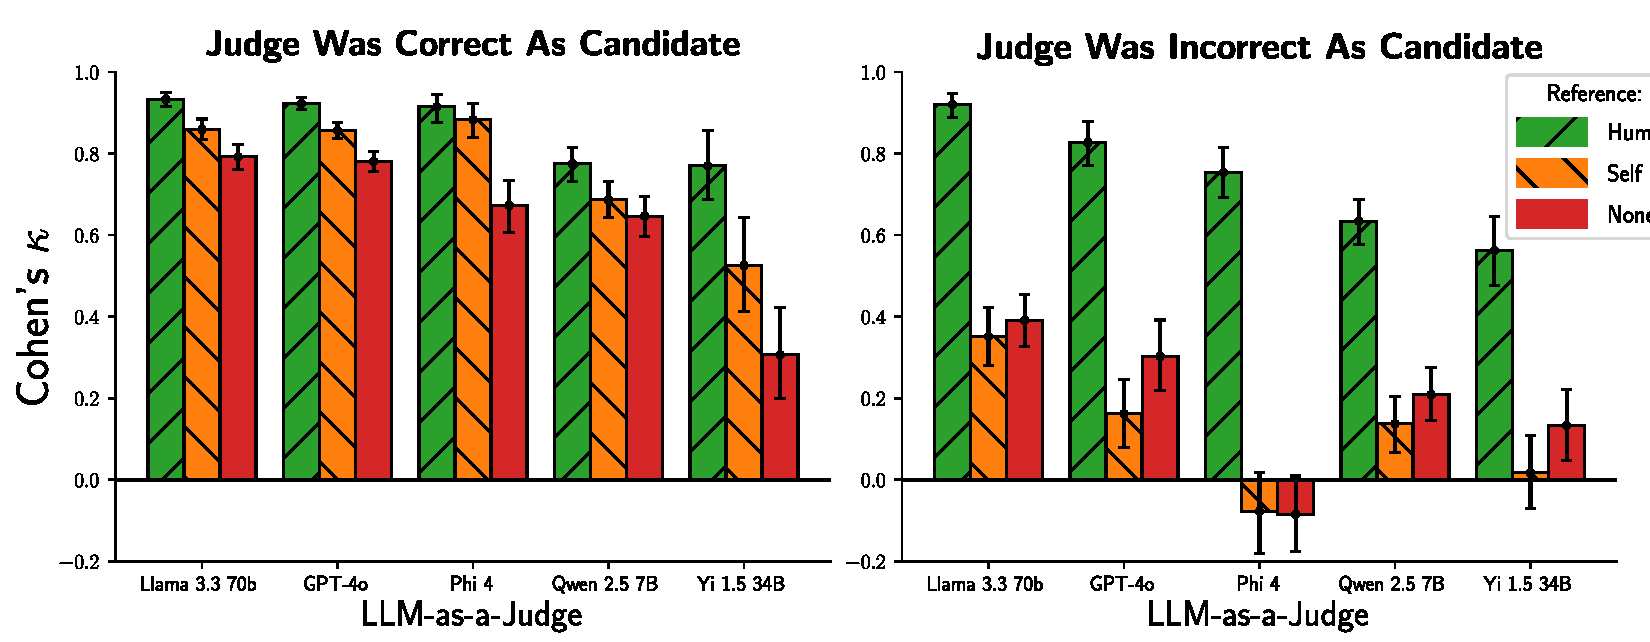
\includegraphics[width=\linewidth]{figures/figure1_plot.pdf}
    \caption{LLM Judge agreement with human annotators for the pairwise correctness judgment task. The left plot shows agreement when using a LLM as a judge on questions it is able to answer correctly, whereas the right plot shows agreement on questions it answers incorrectly. \textit{None} means the judge LLM is provided with no reference response, \textit{Self} means the judge LLM is provided an unverified 
    reference generated by the judge model itself, and \textit{Human} means the judge LLM is provided a human-written gold (correct) reference. When judge LLMs are not provided a correct reference, their agreement with human judgments decreases substantially for responses to questions they cannot correctly answer. However, providing a correct reference recovers much of this agreement.
    }
    \label{fig:one}
\end{figure}
